\documentclass[pdflatex,11pt]{aghdpl}
% \documentclass{aghdpl}               % przy kompilacji programem latex
% \documentclass[pdflatex,en]{aghdpl}  % praca w języku angielskim
\usepackage[polish]{babel}
\usepackage[utf8]{inputenc}

% dodatkowe pakiety
\usepackage{enumerate}
\usepackage{listings}
\usepackage{graphicx}
\usepackage{float}
\lstloadlanguages{TeX}

\lstset{
  literate={ą}{{\k{a}}}1
           {ć}{{\'c}}1
           {ę}{{\k{e}}}1
           {ó}{{\'o}}1
           {ń}{{\'n}}1
           {ł}{{\l{}}}1
           {ś}{{\'s}}1
           {ź}{{\'z}}1
           {ż}{{\.z}}1
           {Ą}{{\k{A}}}1
           {Ć}{{\'C}}1
           {Ę}{{\k{E}}}1
           {Ó}{{\'O}}1
           {Ń}{{\'N}}1
           {Ł}{{\L{}}}1
           {Ś}{{\'S}}1
           {Ź}{{\'Z}}1
           {Ż}{{\.Z}}1
}

%---------------------------------------------------------------------------

\author{Łukasz Zieńkowski}
\shortauthor{Ł. Zieńkowski}

\titlePL{Interaktywna mapa czasu z dodatkową osią czasu}
\titleEN{Thesis in \LaTeX}

\shorttitlePL{Interaktywna mapa czasu z dodatkową osią czasu}
\shorttitleEN{Thesis in \LaTeX}

\thesistypePL{Praca magisterska}
\thesistypeEN{Master of Science Thesis}

\supervisorPL{dr hab. Marcin Szpyrka}
\supervisorEN{Marcin Szpyrka Ph.D}

\date{2011}

\departmentPL{Katedra Automatyki}
\departmentEN{Department of Automatics}

\facultyPL{Wydział Elektrotechniki, Automatyki, Informatyki i Elektroniki}
\facultyEN{Faculty of Electrical Engineering, Automatics, Computer Science and Electronics}

\acknowledgements{Serdecznie dziękuję \dots tu ciąg dalszych podziękowań np. dla promotora, żony, sąsiada itp.}



\setlength{\cftsecnumwidth}{10mm}

%---------------------------------------------------------------------------

\begin{document}

\titlepages

\tableofcontents
\clearpage

\chapter{Wprowadzenie}
\label{cha:wprowadzenie}

2-3 storny\\
cytat (\cite{Dil00}, \cite{Lam92})\\
wyraz $\tau$, $\epsilon$, $\chi$\\
W rodziale~\ref{cha:pierwszyDokument}\\
95\%\\
w pliku \texttt{test.tex}.\\
Na stronie \underline{\texttt{http://kile.sourceforge.net/screenshots.php}}\\
%---------------------------------------------------------------------------

\section{Cele pracy}
\label{sec:celePracy}

%---------------------------------------------------------------------------

\section{Zawartość pracy}
\label{sec:zawartoscPracy}




















\chapter{State of art}
\label{cha:State of art}
20-30
W rozdziale tym przedstawiono podstawowe informacje dotyczące struktury prostych plików \LaTeX a. Omówiono również metody kompilacji plików z zastosowaniem programów \emph{latex} oraz \emph{pdflatex}.

%---------------------------------------------------------------------------

\section{Rodzaje map}
\label{sec:Rodzaje map}

Tworząc aplikację która ma dostarczać informacji korzystających z map należy zapoznać się dostępnymi źródłami. Z powodu szrokiego wyboru poniżej omówione zostaną jedynie aplikacje które dostarczają informacji ogólnoświatowych. Na polskim rynku dostępnych jest kilka rozwiązań, ich główną wadą jest ograniczenie do terytorium Polski, dodatkowo często nie dostarczają one obrazów satelitarnych, są to m.in. \underline{\texttt{http://zumi.pl}}

\subsection{Google Maps}
\label{subsec:Google Maps}

\subsection{Windows Maps}
\label{subsec:Windows Maps}

\subsection{Apple Maps}
\label{subsec:Apple Maps}

\section{Google Earth}
\label{sec:Google Earth}

Ciekawe wykorzystanie obrazów satelitarnych i wskaźnika czasu zostało zaprezentowane w programie Google Earth. W aplikacji tej możemy zobaczyć nie tylko najbardziej aktualne zdjęcia, ale jesteśmy w stanie cofnąć się w czasie i zobaczyć jak wyglądał obszar na który patrzymy w przeszłości.

Przykład takiej sytuacji został przedstawiony na rysunku \ref{fig:lasVegas1}, obraz terenu na którym powstanie miasto Las Vegas w roku 1950. Jak teren ten wyglądał w roku 1977 widzimy na rysunku \ref{fig:lasVegas2}, pomimo widocznych zmian teren ten nadal w dużym stopniu jest pustynny,dopiero na rysunku \ref{fig:lasVegas3} widzimy aktualny stan miasta.

Dzięki funkcji zmiany punktu i kąta patrzenia, pokazywania ciekawych miejsc czy chociażby włączania trybu w którym budynki nabierają formy przestrzennej, 3D, możemy poprzez zabawę i wirtualne wycieczki poszeżać naszą wiedzę o otaczającym nas świecie. 

\begin{figure}[H]
  \centering
    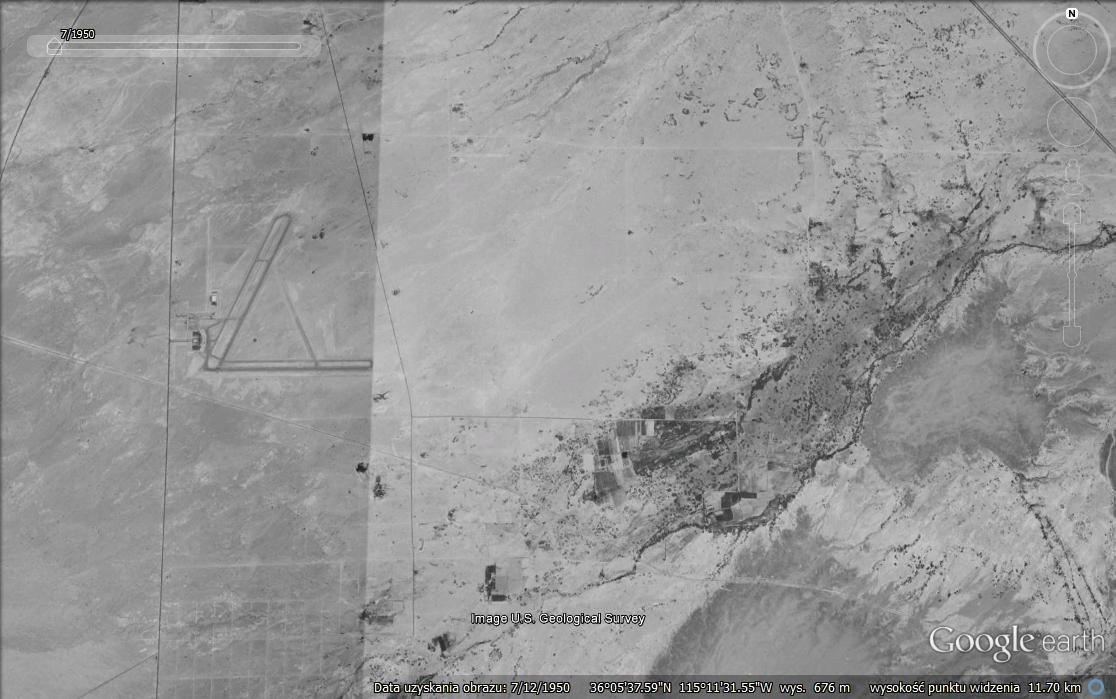
\includegraphics[width=100mm]{ge/01_1950.jpg}
  \caption{Las Vegas w 1950 roku.}
  \label{fig:lasVegas1}
\end{figure}

\begin{figure}[H]
  \centering
    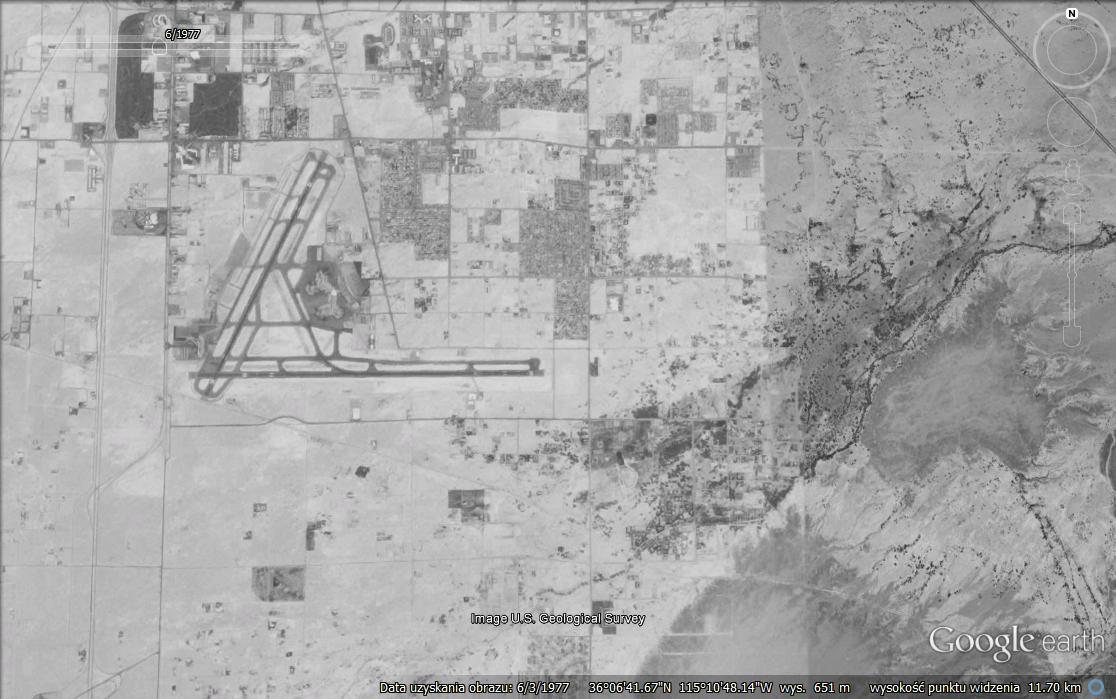
\includegraphics[width=100mm]{ge/02_1977.jpg}
  \caption{Las Vegas w 1950 roku.}
  \label{fig:lasVegas2}
\end{figure}

\begin{figure}[H]
  \centering
    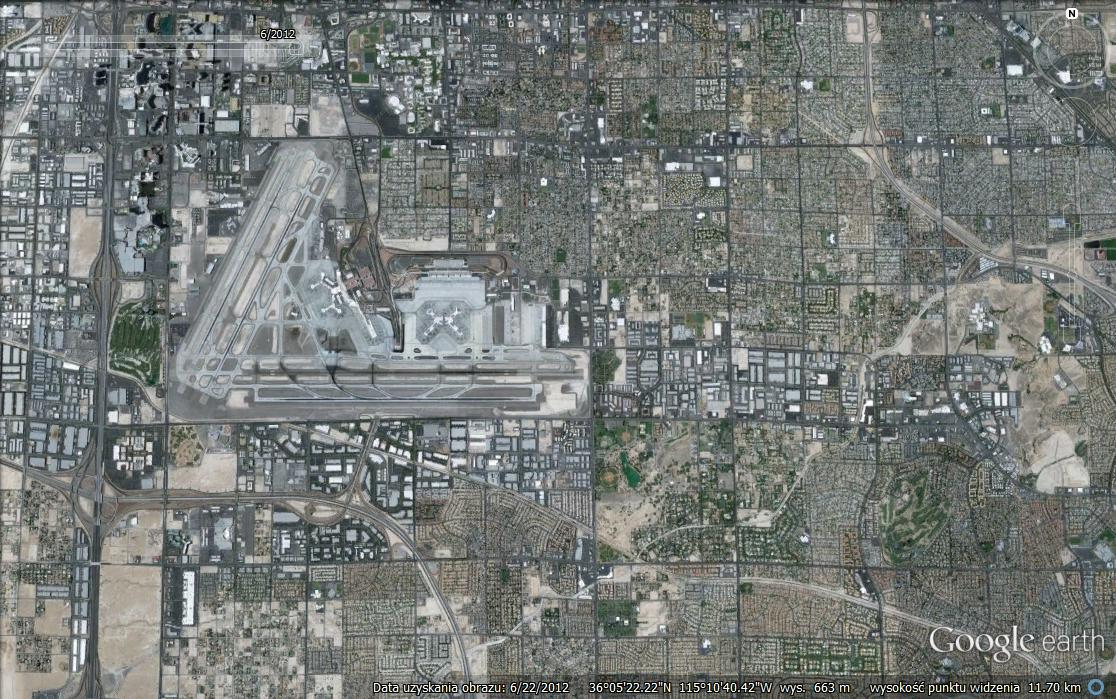
\includegraphics[width=100mm]{ge/03_2012.jpg}
  \caption{Las Vegas w 1950 roku.}
  \label{fig:lasVegas3}
\end{figure}

\section{Time line}
\label{sec:Time line}

Plik \LaTeX owy jest plikiem tekstowym, który oprócz tekstu zawiera polecenia formatujące ten tekst (analogicznie do języka HTML). Plik składa się z dwóch części:
\begin{enumerate}%[1)]
\item Preambuły -- określającej klasę dokumentu oraz zawierającej m.in. polecenia dołączającej dodatkowe pakiety;

\item Części głównej -- zawierającej zasadniczą treść dokumentu.
\end{enumerate}


\begin{lstlisting}
\documentclass[a4paper,12pt]{article}      % preambuła
\usepackage[polish]{babel}
\usepackage[utf8]{inputenc}
\usepackage[T1]{fontenc}
\usepackage{times}

\begin{document}                           % część główna

\section{Sztuczne życie}

% treść
% ąśężźćńłóĘŚĄŻŹĆŃÓŁ

\end{document}
\end{lstlisting}

%---------------------------------------------------------------------------

\section{Kompilacja}
\label{sec:kompilacja}

\begin{lstlisting}
latex test.tex
dvips test.dvi -o test.ps
ps2pdf test.ps
\end{lstlisting}
%
lub za pomocą PDF\LaTeX:
\begin{lstlisting}
pdflatex test.tex
\end{lstlisting}

%---------------------------------------------------------------------------

\section{Narzędzia}
\label{sec:narzedzia}

\begin{itemize}
\item Edit shortcuts -- definiowanie własnych klawiszy skrótu;
\item Line Tools -- dodatkowe operacje na liniach tekstu;
\end{itemize}

%---------------------------------------------------------------------------

\section{Przygotowanie dokumentu}
\label{sec:przygotowanieDokumentu}

Plik źródłowy \LaTeX a jest zwykłym plikiem tekstowym. Przygotowując plik
źródłowy warto wiedzieć o kilku szczegółach:

\begin{itemize}
\item
Poszczególne słowa oddzielamy spacjami, przy czym ilość spacji nie ma znaczenia.
Po kompilacji wielokrotne spacje i tak będą wyglądały jak pojedyncza spacja.
Aby uzyskać {\em twardą spację}, zamiast znaku spacji należy użyć znaku {\em
tyldy}.

\item
Znakiem końca akapitu jest pusta linia (ilość pusty linii nie ma znaczenia), a
nie znaki przejścia do nowej linii.

\item
\LaTeX~sam formatuje tekst. \textbf{Nie starajmy się go poprawiać}, chyba, że
naprawdę wiemy co robimy.
\end{itemize}



\chapter{Definicja problemu}

2-3stony



\chapter{Opis rozwiązania}
\label{cha:Opis rozwiązania}

50%

\section{Transmisja danych}
\label{sec:transmisjaDanych}

xml - 729  557
json - 695  400

\subsection{XML}
\label{subsec:xml}
\lstset{language=XML}
\begin{lstlisting}[caption=caption]
<?xml version="1.0" ?>
<map>
	<title>Tove</title>
	<description>Jani</description>
	<from>123444</from>
	<to>123444</to>
	<markers>
		<marker>
			<x>123.344</x>
			<y>123.344</y>
			<z>123.344</z>
			<from>123444</from>
			<to>123444</to>
			<description>Jani</description>
			<icon>Jani</icon>
		</marker>
		<marker>
			<x>123.344</x>
			<y>123.344</y>
			<z>123.344</z>
			<from>123444</from>
			<to>123444</to>
			<description>Jani</description>
			<icon>Jani</icon>
		</marker>
		<marker>
			<x>123.344</x>
			<y>123.344</y>
			<z>123.344</z>
			<from>123444</from>
			<to>123444</to>
			<description>Jani</description>
			<icon>Jani</icon>
		</marker>
	</markers>
</map>
\end{lstlisting}

\subsection{JSON}
\label{subsec:json}

\lstset{language=JavaScript}
\begin{lstlisting}[caption=json]
{
    "title": "Tove",
    "description": "Jani",
    "from": 123444,
	"to": 123444,
    "markers": [
        {
            "x": "123.344",
			"y": "123.344",
			"z": "123.344",
			"from": "123444",
			"to": "123444",
            "description": "Jani"
            "icon": "Jani"
        },
		{
            "x": "123.344",
			"y": "123.344",
			"z": "123.344",
			"from": "123444",
			"to": "123444",
            "description": "Jani"
            "icon": "Jani"
        },
		{
            "x": "123.344",
			"y": "123.344",
			"z": "123.344",
			"from": "123444",
			"to": "123444",
            "description": "Jani"
            "icon": "Jani"
        },
    ]
}
\end{lstlisting}

\section{Interferjs}
\label{sec:Interferjs}



\chapter{Podsumowanie}

10 %



\chapter{Podsumowanie}

2-3 strony





% itd.
% \appendix
% \include{dodatekA}
% \include{dodatekB}
% itd.

\bibliographystyle{alpha}
\bibliography{bibliografia}
%\begin{thebibliography}{1}
%
%\bibitem{Dil00}
%A.~Diller.
%\newblock {\em LaTeX wiersz po wierszu}.
%\newblock Wydawnictwo Helion, Gliwice, 2000.
%
%\bibitem{Lam92}
%L.~Lamport.
%\newblock {\em LaTeX system przygotowywania dokumentów}.
%\newblock Wydawnictwo Ariel, Krakow, 1992.
%
%\bibitem{Alvis2011}
%M.~Szpyrka.
%\newblock {\em {On Line Alvis Manual}}.
%\newblock AGH University of Science and Technology, 2011.cccccc
%\newblock \\\texttt{http://fm.ia.agh.edu.pl/alvis:manual}.
%
%\end{thebibliography}

\end{document}
